\chapter{ }
\section{Measurment of Time Delay in Video Feedback}
\label{app:DH}
The experiment used to find the time delay in video feedback is described here. The operator station's graphical user interface is shown in Figure \ref{fig:Gui2}. This displays the video received form the camera mounted on the mobile robot  in the window marked with a green boundary.   
\begin{figure}
	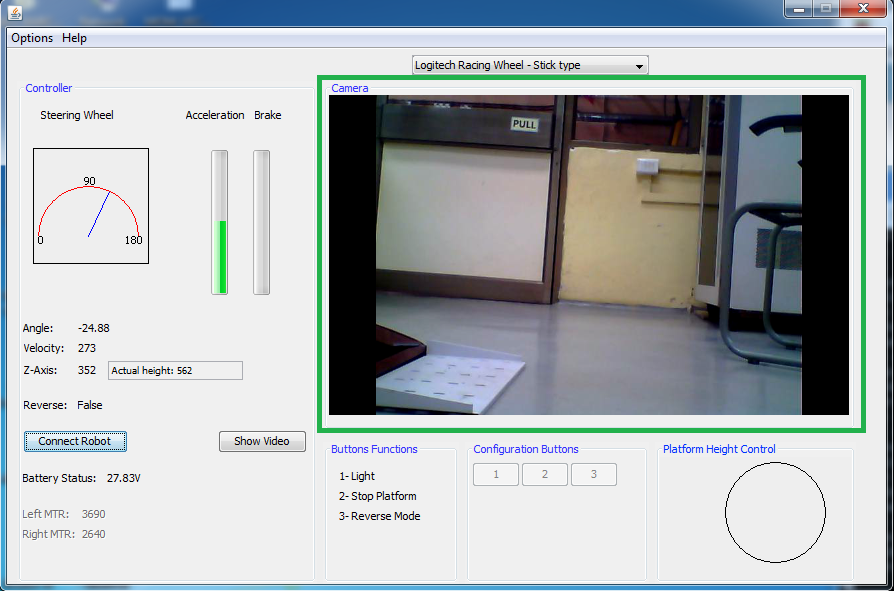
\includegraphics[width=\linewidth,keepaspectratio]{Chapter5/fig/gui1}
	\captionof{figure}{User interface for teleoperation }
	\label{fig:Gui2} 
\end{figure}

To measure the time delay, a digital clock and the user interface runs side by side on the operator screen. The camera on the robot is now oriented to face the user interface, so that the camera captures the video of the digital clock running on the user PC. The schematic of the experimental set-up is shown in Figure \ref{fig:ExptSetup}. The screen shot of the operator screen is shown in Figure \ref{fig:ScreenShot}. The red box marks the clock running on the PC. The blue box marks the time captured by the robot camera in the most recent video frame received at the operator station. We thus see the delay  of $9.2-8.7=0.5$ sec, for the video frame to travel from robot to the operator station. This delay includes both the processing time and the transmission time.

\begin{figure}
	\begin{minipage}[t]{0.6\textwidth}
		\centering
		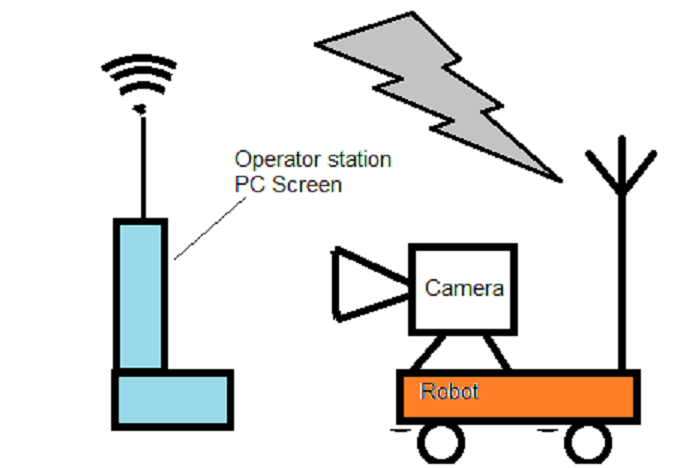
\includegraphics[width=\linewidth,scale=2]{Misc_end/fig/DelayExptSetup2}
		\caption{Experimental setup: Schematic}\label{fig:ExptSetup}
	\end{minipage}
	\hfill
	\begin{minipage}[t]{0.5\textwidth}
		\centering
		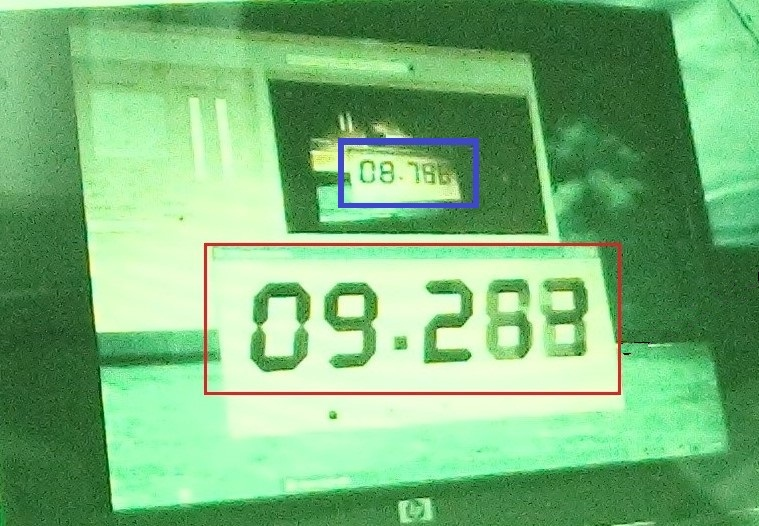
\includegraphics[width=\linewidth]{Misc_end/fig/delayMeasureNew2} 
		\caption{Screen shot of operator PC}\label{fig:ScreenShot}
	\end{minipage}
\end{figure}
% % % % % % % % % % % % % % % % % % % % % % % % %
